\documentclass[sigconf]{acmart}
\usepackage{graphicx}
\usepackage{amsmath}
\usepackage{tikz}
\usetikzlibrary{shapes.geometric, arrows}


\usepackage{booktabs} % For formal tables
%\usepackage{fullpage}
%\usepackage{hyperref}
%\usepackage{authblk}
%\usepackage{caption}
%\usepackage{subcaption}
%\usepackage{listings}
%\lstset{language=python, tabsize=4}

\pdfinfo{
	/Title (Deep Learning Approach to Collaborative Rating Prediction)
}
\title{Deep Learning Approach to Collaborative Rating Prediction}

\begin{document}
\maketitle

\begin{abstract}
	Deep learning has been successful in various domains 
	including image recognition, speech recognition and natural language 
	processing.
	However, the research on its application in recommendation systems is 
	still in an early stage.
	Here we present Model R, a neural network model created to provide a deep 
	learning solution for the collaborative rating prediction problem.
	This model extracts knowledge of users and items from known ratings and 
	uses this knowledge to predict unknown ratings.
	We demonstrate the power of Model R through experiments and compare it with 
	the most prevalent collaborative filtering algorithm - neighborhood-based 
	collaborative filtering.
	Model R shows that deep learning can be successfully applied to 
	collaborative rating prediction and it outperforms neighborhood-based 
	collaborative filtering by up to 18\% in terms of prediction accuracy.
\end{abstract}

\section{Introduction}
The expression deep learning existed as early as 1986 in the machine learning 
community \cite{dechter1986learning}, though not so well known for many 
years.
But now, deep learning techniques using neural network models are rapidly 
gaining traction in more and more application domains such as:
\begin{itemize}
	\item speech recognition \cite{hannun2014deep}
	\item image recognition \cite{simonyan2014very}
	\item natural language processing \cite{yao2013recurrent}
	\item graph mining \cite{grovernode2vec}
	\item recommendation systems \cite{barkan2016item2vec}
\end{itemize}
Two reasons for its adoptions in these domains are its higher prediction 
accuracy and less engineering compared to other machine learning techniques.
Among these domains, research in recommendation systems has been very active  
due to its extremely high value in industries such as search, e-commerce, 
travel and social media \cite{buettner2016predicting}.
Recommendation systems are classified into two groups according to the way they 
extract information about items: content-based filtering and collaborative 
filtering \cite{ricci2011introduction}.
Collaborative filtering extracts information from the relations between users 
and items, while content-based filtering extracts information from the contents 
of items.
There is also a hybrid approach that combines collaborative filtering and 
content-based filtering to get the strengths of both 
\cite{adomavicius2005toward}.
Collaborative filtering has multiple forms including producing a list of items 
a user would like, and predicting the ratings a user would give to a list of 
items \cite{su2009survey}.
The focus of this paper is the rating prediction form of collaborative 
filtering, which we call collaborative rating prediction.
The contribution of this paper is a deep learning approach to collaborative 
rating prediction.

\section{Related work}
In this section,
we review existing deep learning methods in both content-based 
filtering and collaborative filtering.
We also clarify how our work differs from these related works.

\subsection{Content-based filtering methods}
Methods in this group extract information about an item from its content, 
i.e., the input of the neural network is a vector produced from the item's 
content (e.g., the audio of a song, the text of an article). Here are some 
examples:
\begin{itemize}
	\item One example is a music recommendation system 	\cite{van2013deep}. 
	It is a tag prediction system implemented with a convolutional neural net. 
	The input is the spectrogram vector of the audio of a song,
	and the output 	is the set of tags of the song (
	e.g., genre, instrumentation, tempo, mood).
	\item Another example is a multi-view recommendation system 	
	\cite{elkahky2015multi}. 
	It is a rating prediction system implemented with a fully connected 
	neural net.
	The input is the letter tri-gram vector of the text description of an item, 
	etc, and the output is the rating.
	\item A much more comprehensive example is a hierarchical Bayesian model 
	called collaborative deep learning \cite{wang2015collaborative}.
	This approach uses a stacked denoising autoencoder to extract information 
	from the bag-of-word vector of the text description of an item,
	and then uses the extracted information for rating prediction.
\end{itemize}
Similar to image recognition and speech recognition, these methods use deep 
learning to extract information about an entity from the content of the entity.
One of the limitations of content-based filtering is limited content analysis 
\cite{adomavicius2005toward}.
For example, if the items are articles addressing the same topic,
the badly written articles and well-written articles can have very similar 
textual content. In this case, a content-based system will fail to distinguish 
them and give them different ratings.
In this paper, we focus not on content-based filtering, but collaborative 
filtering (i.e., our technique does not access the contents of items).

\subsection{Collaborative filtering methods}
Methods in this group extract information about an item from its relations 
with other items, and the input of the neural net is a vector learned by the 
neural net itself from the relations between items.
These methods treat a list of items as a sentence of words 
(effectively reducing their problems to a natural language processing problem)  
and then apply the skip-gram model used in word2vec 
\cite{mikolov2013efficient}:
\begin{itemize}
	\item An item similarity prediction example is item2vec 
	\cite{barkan2016item2vec} where purchases (lists of items) are 
	treated as sentences.
	\item Similar examples exist in graph mining, like deep walk 
	\cite{perozzi2014deepwalk} and node2vec \cite{grovernode2vec}, 
	where a graph is sampled into walks (lists of nodes),
	and treated as sentences.
\end{itemize}
One drawback of these methods is that they fail to take advantage of 
the highly organized, regular and repeated structure in their relational data: 
relations between users and items (i.e., a user gives numeric rating to an 
item) and relations between nodes (i.e., a source node connects to a 
destination node through a labeled link).
This structure is not exploited in natural language processing because it 
does not exist (i.e., for a neural net, words can simply show up in a sequence 
from a day-to-day conversation, in many flexible and unpredictable ways, with 
little structure or regularity).
Although syntax and semantics exist in natural languages, we have not seen any 
current neural network models taking advantage of these structures.
Our work differs from the above methods in that our technique uses a 
deep learning model designed to take advantage of the structure in the 
relational data and it is also able to predict a numeric attribute - the rating 
value.

\section{Problem}
The problem we consider in this paper is collaborative rating prediction 
problem.
In this section, we look at an example of the problem and then its definition.

\subsection{Problem example}
As an example of a collaborative rating prediction problem, consider 
a set of 6 users who give numeric ratings to a set of 3 items.
For each user, only a subset of their ratings are known; 
and we want to predict the unknown ratings.
The dataset for this example is shown in Table \ref{tab:ratings}.
\begin{table}[!htb]
	\centering
	\caption{Collaborative rating prediction problem example:
		In this dataset, a set of 6 users give ratings to a set of 3 items: 
		for User[0], ratings to all 3 items are known; 
		for User[1], ratings to Item[1] and Item[2] are known, 
		but the rating to Item[0] is unknown; and so on.
		Every unknown rating is marked as a question mark.
		The task is to predict the unknown ratings.
	}
	\begin{tabular}{cccc} \hline
		Ratings & Item[0] & Item[1] & Item[2] \\ \hline
		User[0] & 3       & 5       & 2 \\ \hline
		User[1] & ?       & 5       & 2 \\ \hline
		User[2] & 4       & 4       & 5 \\ \hline
		User[3] & 2       & 4       & ? \\ \hline
		User[4] & 5       & 5       & 4 \\ \hline
		User[5] & 4       & ?       & 4 \\ \hline
	\end{tabular}
	\label{tab:ratings}
\end{table}

\subsection{Problem definition}
Formally, a collaborative rating prediction problem is defined as follows:
\begin{itemize}
	\item Given: a 2-D array R[m][n], 
	where real number R[i][j] is the rating User[i] gives to Item[j],
	integer i $ \in [0, m-1] $, integer j $ \in [0, n-1] $, and a number of 
	p elements in R are unknown
	\item Task: predict all unknown elements in R to minimize MAE.
\end{itemize}
MAE (mean absolute error) is defined as
\begin{align*}
	MAE = \frac{1}{p} \sum_{i = 0}^{p}|f_i - y_i|
\end{align*}
where $ f_i $ is the predicted value, $ y_i $ is the true value, and p is the 
size of test set.
Moreover, we define a user as the array of ratings they give to all items: 
\begin{align*}
	User[i] = R[i]
\end{align*}

\section{Baseline solutions}
Among the many methods for the collaborative rating prediction problem,
the most prevalent one is the neighborhood-based collaborative filtering 
algorithm \cite{su2009survey}.
This algorithm also has several variants,
which we will use as baseline solutions.

\subsection{Algorithm}
The neighborhood-based collaborative filtering algorithm calculates each 
unknown R[i][j] as 
follows \cite{su2009survey}:
\begin{align*}
R[i][j] = c \sum_{k = 0}^{m-1} S(i, k) R[k][j]
\end{align*}
where S(i, k) is the similarity of User[i] and User[k] to be defined by each 
variant,
unknown R[k][j]'s are omitted and c is a normalizing factor:
\begin{align*}
	c = \frac{1}{\sum_{l = 0}^{m - 1} |S(i, k)|}
\end{align*}
It is easy to understand the predicted rating R[i][j] as the sum of ratings all 
users give to Item[j],
weighted by how similar each user is to the target user.
The algorithm can opt to use only a fixed number of users with highest 
similarities to the target user in the calculation, instead of using all users.

\subsection{Variants}
Each variant of the algorithm has a unique definition of the similarity 
function of User[i] and User[k]:
\begin{itemize}
	\item PCC: The Pearson correlation coefficient similarity, defined as 
	\cite{resnick1994grouplens}:
	\begin{align*}
		& S_{PCC}(x, y) \\
		=& \frac{\sum_{i \in I_{xy}}(R[x][i] - \overline{R[x]})(R[y][i] - 
		\overline{R[y]})}{\sum_{i \in I_{xy}}(R[x][i] - \overline{R[x]})^2 
		\sum_{i 
		\in I_{xy}}(R[y][i] - \overline{R[y]})^2 }
	\end{align*}
	where $ I_{x} $ is the set of items rated by User[x],
	and	$ \overline{R[x]} $ is the average rating User[x] gives to all items,
	and $ I_{xy} $ is the set of items rated by both User[x] and User[y].
	PCC measures the linear correlation of two users.
	\item WPCC: The weighted PCC similarity, defined as 
	\cite{herlocker1999algorithmic}:
	\begin{align*}
		S_{WPCC}(x, y)=
		\begin{cases}
			\frac{|I_{xy}|}{T} S_{PCC}(x, y) & |I_{xy}| < T \\
			S_{PCC}(x, y) & otherwise
		\end{cases}
	\end{align*}
	where T is a threshold of number of items. 
	WPCC of two users differs from PCC only when the number of items rated by 
	both users (co-rated items) is less than the threshold. 
	When the difference occurs, fewer co-rated items results in less similarity 
	between the two users.
	\item SPCC: The sigmoid PCC similarity, defined as 	
	\cite{jamali2009trustwalker}:
	\begin{align*}
		S_{SPCC} (x, y)
		= \frac{S_{SPCC}(x, y)}{1 + exp(-\frac{|I_{xy}|}{2})}
	\end{align*}
	SPCC is very similar to WPCC in the sense two users have lower similarity 
	if they have a smaller number of co-rated items.
	\item MPCC: The multi-level PCC similarity \cite{polatidis2016multi}. 
	This one is also very similar to the previous ones but much more complex.
	MPCC essentially uses the PCC similarity measure, but increases it 
	based on the number of co-rated items between the two users,
	as long as the PCC similarity is sufficiently high.
	The more co-rated items, the larger the increase.
	But if the number of co-rated items or the PCC similarity is too low,
	then a similarity of zero is returned.
\end{itemize}

\section{Observations}
Although the methods described in the related work section cannot solve the 
collaborative rating prediction problem,
they all have an interesting key process: representing entities as vectors.
As deep learning techniques become more powerful and standardized, this key 
process seems to be the most significant part in a domain-specific deep 
learning approach.
Here we take a similar approach.

\subsection{Entities and representations}
First of all, we summarize how a neural net represents various types of 
entities in different domains with different relations, as shown in 
Table \ref{tab:domains}.
It is clear that representations for all the entities are numeric arrays, 
because neural nets rely on neurons' activations and communications, which 
are both numeric.
\begin{table}[!htb]
	\centering
	\caption{A summary of various types of entities, their numeric
		representations and inter-entity relations in different domains:
		An image in image recognition is represented as a 2D light amplitude 
		array with dimensions height and width; an audio in speech recognition 
		is represented as a 2D sound amplitude array with dimensions time and 
		frequency.
		The relation between two images or two audio is not commonly used. 
		Words in natural languages, items in recommendation systems, and nodes 
		in graphs can be represented by vectors (1D numeric arrays).
		The	relations between two words, two items and two nodes are commonly 
		used to learn these vectors.
	}
	\begin{tabular}{ccc} \hline
		Entity & Representation               & Relations \\ \hline
		image  & 2D array[width, height]      & N/A \\ \hline
		audio  & 2D array[time, frequency]    & N/A \\ \hline
		word   & 1D array (i.e., word vector) & co-occurrences \\ \hline
		item   & 1D array (i.e., item vector) & co-purchases \\ \hline
		node   & 1D array (i.e., node vector) & connections \\ \hline
	\end{tabular}
	\label{tab:domains}
\end{table}

\subsection{Entities to vectors}
The word2vec technique is famous for using a neural net to learn to map every 
entity (word in this case) in a vocabulary to a vector without any domain 
knowledge \cite{mikolov2013efficient}.
The subsequent techniques item2vec and node2vec use the same skip-gram 
model used in word2vec to map items and nodes to vectors.
In a corpus, every word is described/defined only by related words in its 
contexts, by implicit relations between words in word co-occurrences.
Nonetheless, the neural net can learn from word co-occurrences and map words to 
vectors accordingly,
such that the relations between words are preserved in the word vector space 
\cite{mikolov2013distributed}.
The same arguments apply to relations between items and between nodes.

\subsection{Users and items to vectors}
However, the relation between a user and an item is quite different from that 
between words:
\begin{itemize}
	\item The rating a user gives to an item explicitly tells us how much the 
	user likes that item;
	the relation is very specific: one user, one item, one rating.
	\item The co-occurrences of words [quick, brown, fox, jumps, over] 
	implicitly tell us these words are related but do not tell us any 
	specific 
	relation.
\end{itemize}
This observation suggests that a neural net should be able to learn a 
user-to-vector mapping and an item-to-vector mapping supervised by the rating,
in a more specific, direct and simply way than it learns word-to-vector 
mappings supervised by word co-occurrences.

\section{Solution}
Following the above observations, we can build an estimator with a neural net 
model using a (user, item) pair as its input and the rating as its output.
Therefore, we should change the format of the example dataset from the one 
shown in Table \ref{tab:ratings} to a new one shown in Table \ref{tab:rating}.
The estimator will train on entries with known ratings (the training set) 
and predict on the entries with unknown ratings (the test set).
Of course our testing program knows the unknown ratings in order to calculate 
the model's prediction error.
\begin{table}[!htb]
	\centering
	\caption{The reformatted dataset of the problem example.}
	\begin{tabular}{cc}  \hline
		Input = (User ID, Item ID) & Output = Rating \\ \hline
		(0, 0)                     & 3 \\ \hline
		(0, 1)                     & 5 \\ \hline
		(0, 2)                     & 2 \\ \hline
		(1, 0)                     & ? \\ \hline
		(1, 1)                     & 5 \\ \hline
		(1, 2)                     & 2 \\ \hline
		...                        & ... \\ \hline
		(5, 2)                     & 4 \\ \hline
	\end{tabular}
	\label{tab:rating}
\end{table}

\subsection{Conceptual deep learning model}
The model in the estimator is a fully connected neural net which we call Model 
R (R as in relation), shown in Figure \ref{fig:conceptural}.
\begin{figure*}[!htb]
	\centering
	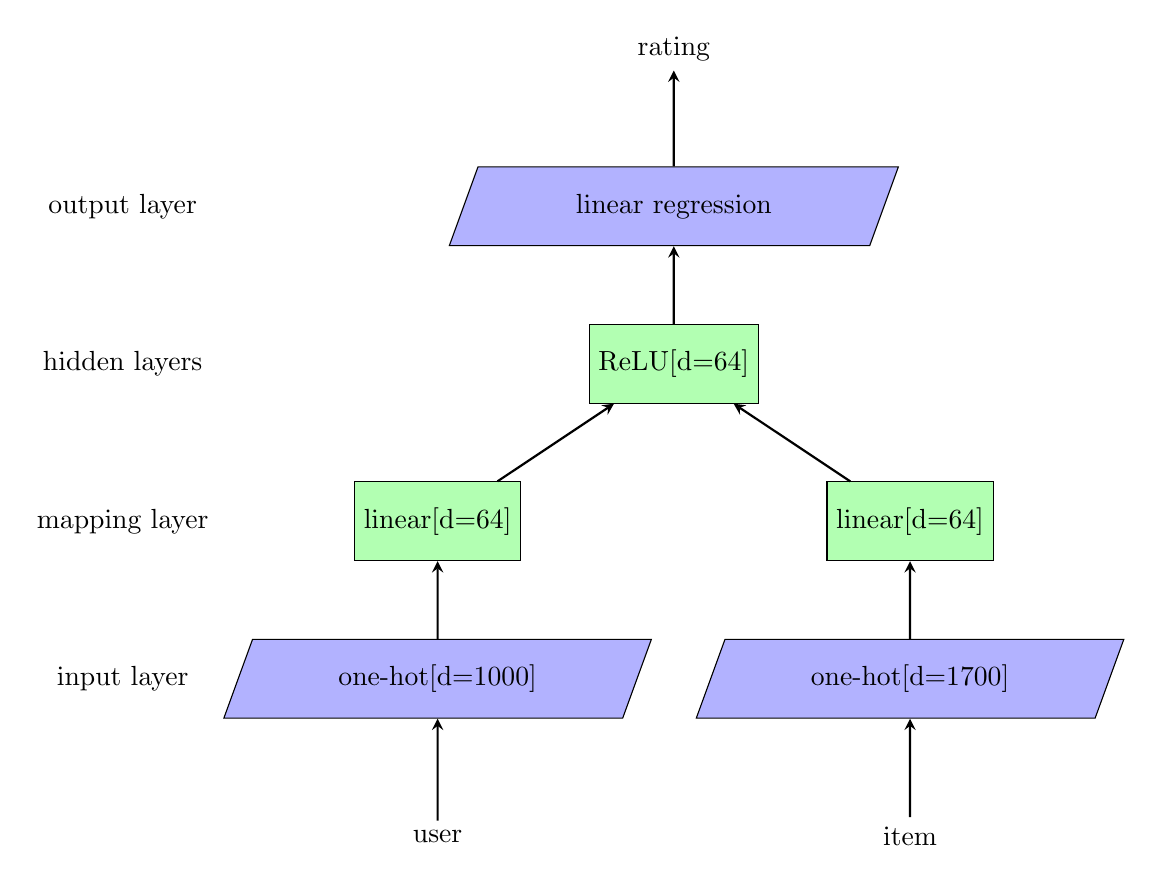
\begin{tikzpicture}[node distance=2cm]
	\tikzstyle{io} = [trapezium, trapezium left angle=70, trapezium right 
	angle=110, minimum width=1cm, minimum height=1cm, text centered, 
	draw=black, fill=blue!30]
	\tikzstyle{process} = [rectangle, minimum width=1cm, minimum height=1cm, 
	text centered, draw=black, fill=green!30]
	\tikzstyle{arrow} = [thick,->,>=stealth]
	\node (linearRegression) [io] {linear regression};
	\node (relu3) [process, below of=linearRegression] {ReLU[d=64]};
	\node (linear1) [process, below of=relu3, xshift=-3cm] {linear[d=64]};
	\node (linear2) [process, below of=relu3, xshift=3cm] {linear[d=64]};
	\node (oneHot2) [io, below of=linear2] {one-hot[d=1700]};
	\node (oneHot1) [io, below of=linear1] {one-hot[d=1000]};
	\node (rating) [above of=linearRegression] {rating};
	\node (output) [left of=linearRegression, xshift=-5cm] {output layer};
	\node (hidden1) [below of=output] {hidden layers};
	\node (mapping) [below of=hidden1] {mapping layer};
	\node (input) [below of=mapping] {input layer};
	\node (user) [below of=oneHot1] {user};
	\node (item) [below of=oneHot2] {item};
	\draw [arrow] (user) -- (oneHot1);
	\draw [arrow] (item) -- (oneHot2);
	\draw [arrow] (oneHot1) -- (linear1);
	\draw [arrow] (oneHot2) -- (linear2);
	\draw [arrow] (linear1) -- (relu3);
	\draw [arrow] (linear2) -- (relu3);
	\draw [arrow] (relu3) -- (linearRegression);
	\draw [arrow] (linearRegression) -- (rating);
	\end{tikzpicture}
	\caption{The conceptual model R for a dataset with 1700 items and 1000 
		users:
		The d in the bracket (d as in dimension) is the layer's size (number of 
		units in the layer).
		We keep all non-input layers the same size for simplicity, although 
		layers of different sizes may produce better results.
		The text before the bracket refers to the activation function of the 
		units in the layer (except for one-hot, which refers to the activations 
		in the input layer).
		Only layers and their connections are shown, while the units in each 
		layer and their connections are not shown.
	}
	\label{fig:conceptural}
\end{figure*}
The model contains the following layers:
\begin{itemize}
	\item An input layer with one-hot activations.
	It has 1 channel for items and 1 channel for users.
	This layer is directly activated by the testing program (
	e.g., to feed the 1200th item, the testing program sets 1 at the 1200th 
	unit and 0 at other units in the item channel).
	\item A mapping layer with linear units. It has one channel to map each 
	entity to a vector.
	The activations of these two channels are the two vectors.
	It is the most critical layer as it gradually learns to map users and 
	items to vectors,
	which are complex and unobservable user and item attributes.
	\item Multiple fully connected hidden layers (only one layer is shown in the
	figure, but	multiple numbers of layers and layer sizes are evaluated in 
	the experiments) of ReLU (rectified linear units).
	These units have non-linear activation functions to give the model 
	sufficient complexity.
	These layers learn to extract more and more abstract rating-relevant 
	information.
	\item An output layer with a linear regression unit.
	It learns to predict the rating based on abstracted information.
\end{itemize}
In this problem, ratings provide the information about users and items.
We fully take this property into account and design this model to learn 
complex and unobservable user and item attributes (i.e., user and item vectors) 
supervised by a simple observable rating.

\subsection{Actual deep learning model}
In practice, Model R uses more efficient mapping tables instead of a 
one-hot input layer in order to handle a dataset with an increasing number of 
users and items, as shown in Figure \ref{fig:actural}.
The actual model has with two modifications from the conceptual model:
\begin{itemize}
	\item The input layer is replaced by two mapping tables: one for users and 
	one for items.
	Their inputs are user and item IDs and their outputs are user and item 
	vectors.
	\item The mapping layer is replaced by a 2-channel input layer. It is 
	directly activated by the outputs of the mapping tables.
\end{itemize}
\begin{figure*}[!htb]
	\centering
	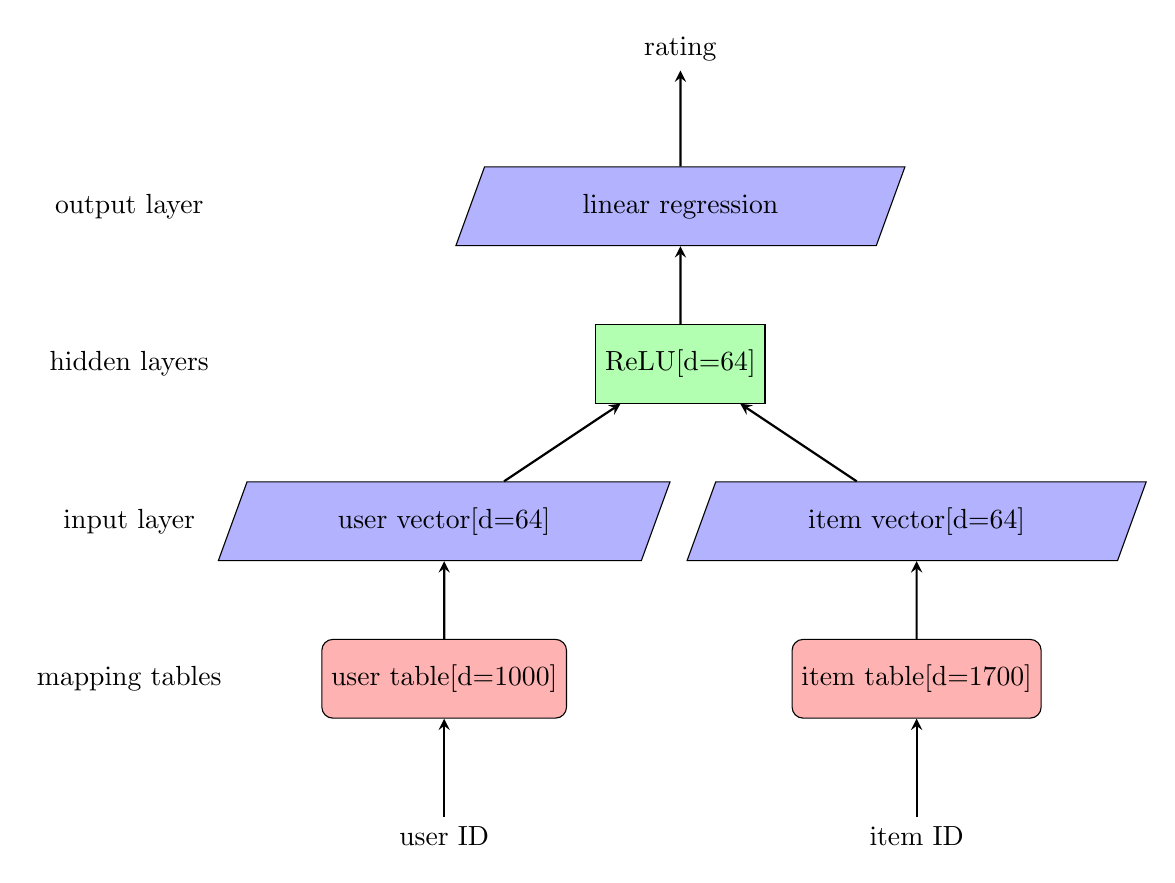
\begin{tikzpicture}[node distance=2cm]
	\tikzstyle{io} = [trapezium, trapezium left angle=70, trapezium right 
	angle=110, minimum width=1cm, minimum height=1cm, text centered, 
	draw=black, fill=blue!30]
	\tikzstyle{startstop} = [rectangle, rounded corners, minimum width=1cm, 
	minimum height=1cm, text centered, draw=black, fill=red!30]
	\tikzstyle{process} = [rectangle, minimum width=1cm, minimum height=1cm, 
	text centered, draw=black, fill=green!30]
	\tikzstyle{arrow} = [thick,->,>=stealth]
	\node (linearRegression) [io] {linear regression};
	\node (relu3) [process, below of=linearRegression] {ReLU[d=64]};
	\node (linear1) [io, below of=relu3, xshift=-3cm] {user vector[d=64]};
	\node (linear2) [io, below of=relu3, xshift=3cm] {item vector[d=64]};
	\node (oneHot1) [startstop, below of=linear1] {user table[d=1000]};
	\node (oneHot2) [startstop, below of=linear2] {item table[d=1700]};
	\node (rating) [above of=linearRegression] {rating};
	\node (output) [left of=linearRegression, xshift=-5cm] {output layer};
	\node (hidden1) [below of=output] {hidden layers};
	\node (input) [below of=hidden1] {input layer};
	\node (mapping) [below of=input] {mapping tables};
	\node (user) [below of=oneHot1] {user ID};
	\node (item) [below of=oneHot2] {item ID};
	\draw [arrow] (user) -- (oneHot1);
	\draw [arrow] (item) -- (oneHot2);
	\draw [arrow] (oneHot1) -- (linear1);
	\draw [arrow] (oneHot2) -- (linear2);
	\draw [arrow] (linear1) -- (relu3);
	\draw [arrow] (linear2) -- (relu3);
	\draw [arrow] (relu3) -- (linearRegression);
	\draw [arrow] (linearRegression) -- (rating);
	\end{tikzpicture}
	\caption{The actual model with two modifications:
		We factor the entity vector mapping process out of the neural net into 
		2 mapping tables.
		We feed every item or user to the estimator by feeding the ID.
		During learning, the estimator updates the vectors in the tables the 
		same way it updates weights in the conceptual model.}
	\label{fig:actural}
\end{figure*}

\subsection{Learning techniques}
The estimator uses the above model and a number of popular deep learning 
techniques:
\begin{itemize}
	\item Backpropagation: propagation of the error gradients from output layer 
	back to each earlier layer \cite{rumelhart1988learning}
	\item Stochastic gradient descent: the optimization that minimizes 
	the error (descending against the error gradient in weight space) for a 
	random sample in each gradient decent step \cite{lecun2012efficient}
	\item Mini-batch: the modification to stochastic gradient descent to 
	accelerate and smooth the descent by minimizing the error for a small 
	random batch of samples in each gradient decent step \cite{mairal2010online}
\end{itemize}

\section{Experiments}
We evaluated Model R and the baseline solutions experimentally,
and the results show that Model R achieved much lower prediction error than 
the baseline solutions.

\subsection{Experiment settings}
We evaluated Model R in the same settings used in a recent experimental 
evaluation of the baseline solutions \cite{polatidis2016multi} on four datasets:
\begin{itemize}
	\item ML100K: MovieLens100K\cite{harper2015movielens}
	\item ML1M: MovieLens1M\cite{harper2015movielens}
	\item EP: Epinions \cite{massa2007trust}
	\item MT: MovieTweetings \cite{dooms2013movietweetings}
\end{itemize}
The specifications of the datasets are summarized in Table \ref{tab:dataset}.
The experiments use MAE as the prediction accuracy metric,
and split each dataset randomly into 2 parts: 20\% into the test set and 80\% 
into the training set.
\begin{table}[!htb]
	\centering
	\caption{The dataset specs: 
		The three columns are the dataset, number of users, items and ratings 
		of the dataset.
		}
	\begin{tabular}{cccc}  \hline
		Dataset & Users   & Items   & Ratings \\ \hline
		ML100K  & 1,000   & 1,700   & 100,000 \\ \hline
		ML1M    & 6,000   & 4,000   & 1,000,000 \\ \hline
		EP      & 49,290  & 139,738 & 664,824 \\ \hline
		MT      & 39,363  & 22,610  & 431,780 \\ \hline
	\end{tabular}
	\label{tab:dataset}
\end{table}

\subsection{Experiment process}
At the beginning of an experiment on a dataset,
the estimator sets aside 10\% of the training set as a validation set.
A larger or smaller validation set did not reduce the prediction error in the 
experiments.
Then the estimator learns for several epochs:
in each epoch,
it learns on the training set,
predicts on the validation set,
and logs the validation error.
In order to reduce over-fitting,
the estimator stops learning when the validation error has not decreased for 3 
epochs.
At the end, the testing program lets the estimator predict on the test set 
and record its testing error as its prediction error on that dataset.

\subsection{Experiment results}
In our experiments, Model R's prediction error is 18\% to 8\% lower than
the best baseline solution (i.e., MPCC) on all datasets, as shown in Table 
\ref{tab:errors}.
The error reduction from MPCC to Model R is calculated as:
\begin{align*}
	\delta = \frac{MPCCError - ModelRError}{MPCCError}
\end{align*}
\begin{table}[!htb]
	\centering
	\caption{The comparison of prediction errors (measured by MAE): 4 baseline
		solutions are represented by their first letters (P, W, S, M).
		Model R's (represented by letter R) prediction error is 18\% to 8\% 
		lower than the best baseline 
		solution (MPCC) on all datasets.
		}
	\begin{tabular}{ccccccc} \hline
		Dataset & P    & W    & S    & M    & R    & $ \delta $ \\ \hline
		ML100K  & 0.83 & 0.82 & 0.83 & 0.82 & 0.69 & 16\% \\ \hline
		ML1M    & 0.83 & 0.81 & 0.83 & 0.79 & 0.65 & 18\% \\ \hline
		EP      & 1.00 & 1.02 & 1.00 & 0.93 & 0.76 & 18\% \\ \hline
		MT      & 1.38 & 1.32 & 1.33 & 1.26 & 1.15 & 9\%  \\ \hline
	\end{tabular}
	\label{tab:errors}
\end{table}
Model R is also very robust in a wide range of parameter settings, shown in 
Table \ref{tab:robust}.
\begin{table}[!htb]
	\centering
	\caption{High robustness of Model R against parameter changes:
		The estimator maintains its prediction error in range [0.68, 0.73] for 
		a wide range of parameter settings. The batch size is the size of the 
		batch of samples used in a single gradient decent step.
		These experiments are on MovieLens 100K dataset with learning rate set 
		at 0.01.
	}
	\begin{tabular}{cccc}  \hline
		 batch size & layer size & hidden layers \# & MAE \\ \hline
		 16 & 16 & 2 & 0.714 \\ \hline
		 16 & 16 & 8 & 0.710 \\ \hline
		 16 & 64 & 2 & 0.687 \\ \hline
		 16 & 64 & 8 & 0.706 \\ \hline
		 64 & 16 & 2 & 0.703 \\ \hline
		 64 & 16 & 8 & 0.724 \\ \hline
		 64 & 64 & 2 & 0.703 \\ \hline
		 64 & 64 & 8 & 0.713 \\ \hline
	\end{tabular}
	\label{tab:robust}
\end{table}
\subsection{Computing resources}
We ran our experiments on a Dell Optiplex 780 machine with Ubuntu 16.04 64-bit 
operating system, Intel Core 2 Duo CPU E8400 @ 3GHz processor and 4 GB memory.
Each run (learning and prediction) takes 2 to 8 minutes,
depending on the dataset and parameters.
Our implementation exploits thread level parallelism, but we have not explored 
data level parallelism (i.e., GPU) or process level parallelism (e.g., 
distributed cluster).

\section{Future work}
We designed Model R for the collaborative rating prediction problem,
but we would like to incorporate a content-based capability to improve its 
prediction accuracy.
For example, in order to better predict the rating a user gives to an article,
the model can append units at the mapping layer to receive a content vector 
mapped from the text of the article by another neural net.
The model can also append one unit for each numeric attribute of the user or 
item (e.g., the age of a user, the price of a product) at the mapping layer.
In this way, it will take advantage of not only relation data but also content 
data, and therefore make more accurate predictions.
We have an open source Python implementation under MIT license hosted on Github 
(url omitted to comply with AAAI review requirements).
The main machine learning package we use is TensorFlow 
\cite{abadi2016tensorflow}.

\section{Conclusions}
Model R shows that deep learning can be successfully applied to the 
collaborative rating prediction problem
and it can achieve higher prediction accuracy than a state-of-the-art 
collaborative filtering method.
The estimator powered by Model R effectively learns complex and unobservable 
user and item attributes from simple and observable relations (i.e., users rate 
items).
The estimator learns both to map each entity to a vector, and to predict 
the rating using these vectors.

\bibliographystyle{aaai}
\bibliography{references}
\end{document}
